\documentclass[a4paper,14pt]{article}

\usepackage{comment} % Para comentar várias linhas ao mesmo tempo

%matemática
\usepackage{amsmath}
\usepackage{amssymb}

%diagramação
\usepackage{extsizes}
\everymath{\displaystyle}
\usepackage{geometry}
\usepackage{fancyhdr}
\usepackage{multicol}
\usepackage{graphicx}
\usepackage[brazil]{babel}
\usepackage[shortlabels]{enumitem}
\usepackage{cancel}
\usepackage{textcomp}
\usepackage{tcolorbox}

%tabelas
\usepackage{array} % Para melhor formatação de tabelas
\usepackage{longtable}
\usepackage{booktabs}  % Para linhas horizontais mais bonitas
\usepackage{float}   % Para usar o modificador [H]
\usepackage{caption} % Para usar legendas em tabelas
\usepackage{wrapfig} % Para usar tabelas e figuras flutuantes


%tikzpicture
\usepackage{tikz}
\usepackage{scalerel}
\usepackage{pict2e}
\usepackage{tkz-euclide}
\usetikzlibrary{calc}
\usetikzlibrary{patterns,arrows.meta}
\usetikzlibrary{shadows}
\usetikzlibrary{external}

%pgfplots
\usepackage{pgfplots}
\pgfplotsset{compat=newest}
\usepgfplotslibrary{statistics}
\usepgfplotslibrary{fillbetween}

%colours
\usepackage{xcolor}



\columnsep=2cm
\hoffset=0cm
\textwidth=8cm
\setlength{\columnseprule}{.1pt}
\setlength{\columnsep}{2cm}
\renewcommand{\headrulewidth}{0pt}
\geometry{top=1in, bottom=1in, left=0.7in, right=0.5in}

\pagestyle{fancy}
\fancyhf{}
\fancyfoot[C]{\thepage}

\begin{document}
	
	\noindent\textbf{6FMA05 - Matemática} 
	
	\begin{center}Formas descritivas (Versão estudante)
	\end{center}
	
	\noindent\textbf{Nome:} \underline{\hspace{10cm}}
	\noindent\textbf{Data:} \underline{\hspace{4cm}}
	
	%\section*{Questões de Matemática}
	
	\begin{multicols}{2}
		\noindent Há infinitas formas de nos referirmos ao número 2: \\
		2; 1 + 1; 3 - 1; (1 + 1) $\cdot$ 1; $\frac{6}{3}$; 0 + 2; etc. \\
		Todas essas maneiras são \textbf{descrições} do número 2. \\
		\textbf{Forma descritiva} é uma descrição ou uma forma descritiva com variável. \\
		Exemplos de formas descritivas com variáveis: \\
		$x; 1 + k; x - y; a + b + c;$ etc.
		\noindent\textsubscript{-----------------------------------------------------------------------}
		\begin{enumerate}
			\item Apresente seis descrições do número 5. \\\\\\\\\\\\\\
			\item A partir de cada descrição que você fez no exercício 1, obtenha uma forma descritiva com uma variável. Use letras diferentes para cada caso. \\\\\\\\\\\\
			\item Quando possível, a partir de cada descrição do exercício 1, obtenha uma forma descritiva com duas variáveis distintas. \\\\\\\\\\\\\\\\\\\
			\item A figura abaixo representa uma calculadora com várias teclas faltando. Usando apenas os botões dessa calculadora, apresente pelo menos uma forma descritiva dos números 6, 7, 8, 10, 12, 15, 17, 30 e 50. \\
			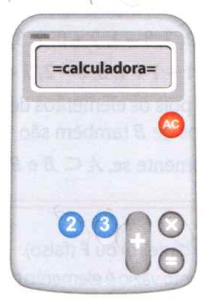
\includegraphics[width=0.7\linewidth]{6FMA05_imagens/imagem1} \newpage
			%16 a 18
			\item Escreva quatro descrições do número 8. \\\\\\\\\\\\\\\\\\\
			\item Escreva cinco descrições do número 6. A partir de cada uma delas, obtenha uma forma descritiva com uma variável. Use letras diferentes para cada um dos casos. \\\\\\\\\\\\\\\\\\\
			\item Das expressões abaixo, assinale quais são formas descritivas.
			\begin{enumerate}[a)]
				\item 7
				\item 9 - 3 = 6
				\item 3 -
				\item $a + b + c$
				\item $a = 6$
				\item $5a$
			\end{enumerate}
		\end{enumerate}
		$~$ \\ $~$ \\ $~$ \\ $~$ \\ $~$ \\ $~$ \\ $~$ \\ $~$ \\ $~$ \\ $~$ \\ $~$ \\ $~$ \\ $~$ \\ $~$ \\ $~$ \\ $~$ \\ $~$ \\ $~$ \\ $~$ \\ $~$ \\ $~$ \\ $~$ \\ $~$ \\ $~$ \\ $~$ \\ $~$ \\ $~$ \\ $~$ \\ $~$ \\ $~$ \\ $~$ \\ $~$ \\ $~$ \\ $~$ \\ $~$ \\ $~$ \\ $~$ \\ $~$ \\ $~$ \\ $~$ \\ $~$ \\ $~$ \\ $~$ \\ $~$ \\ 
	\end{multicols}
\end{document}